\documentclass[crop,tikz]{standalone}
\usepackage{pgfplots}
\pgfplotsset{compat=1.13}

\pgfplotsset{
  inverted/.style = {
    every axis legend/.append style={
      draw=white,
      fill=hardblack,
      text=white
    }
  },
  every non boxed x axis/.append style={
    axis line style={-latex}
  },
  every non boxed y axis/.append style={
    axis line style={-latex}
  }
}

\begin{document}
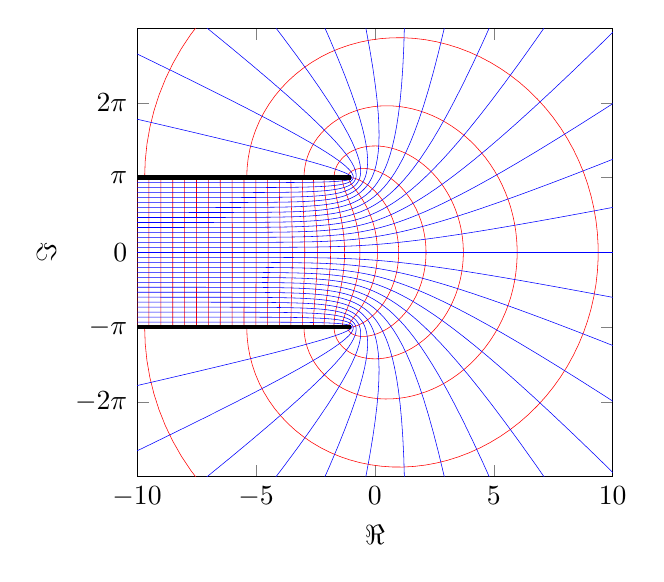
\begin{tikzpicture}
  \pgfmathsetmacro{\numberoffieldlines}{40};
  \pgfmathsetmacro{\numberofpotentiallines}{30};
  \pgfmathsetmacro{\remin}{-10};
  \pgfmathsetmacro{\remax}{10};
  \pgfmathsetmacro{\immin}{-3*pi};
  \pgfmathsetmacro{\immax}{3*pi};
  \begin{axis}[
    axis equal image,
    xmin={\remin}, xmax={\remax},
    ymin={\immin}, ymax={\immax},
    ytick={-2*pi,-pi,0,pi,2*pi},
    yticklabels={$-2\pi$,$-\pi$,$0$,$\pi$,$2\pi$},
    xlabel={$\Re$},
    ylabel={$\Im$},
    samples=100,
    ]
    % field lines
    \pgfplotsinvokeforeach{{\remin},{\remin - \remin*2/\numberoffieldlines},...,5}{
      \addplot[red,very thin,domain={-pi}:{pi}] ({#1 + exp(#1)*cos(deg(x))},{x + exp(#1)*sin(deg(x))});
    }
    % lines of constant potential
    \pgfplotsinvokeforeach{{-\numberofpotentiallines/2},...,{\numberofpotentiallines/2}}{
      \addplot[blue,very thin,domain={\remin}:3] ({x + exp(x)*cos(#1*360/\numberofpotentiallines)},{#1*2*pi/\numberofpotentiallines + exp(x)*sin(#1*360/\numberofpotentiallines)});
    }
    % capacitor plates
    \addplot[domain={\remin}:-1,ultra thick] { pi};
    \addplot[domain={\remin}:-1,ultra thick] {-pi};
  \end{axis}
\end{tikzpicture}
\end{document}
